% A LaTeX template for EXECUTIVE SUMMARY of the MSc Thesis submissions to 
% Politecnico di Milano (PoliMi) - School of Industrial and Information Engineering
%
% S. Bonetti, A. Gruttadauria, G. Mescolini, A. Zingaro
% e-mail: template-tesi-ingind@polimi.it
%
% Last Revision: October 2021
%
% Copyright 2021 Politecnico di Milano, Italy. NC-BY

\documentclass[11pt,a4paper,twocolumn]{article}

%------------------------------------------------------------------------------
%	REQUIRED PACKAGES AND  CONFIGURATIONS
%------------------------------------------------------------------------------
% PACKAGES FOR TITLES
\usepackage{titlesec}
\usepackage{color}

% PACKAGES FOR LANGUAGE AND FONT
\usepackage[utf8]{inputenc}
\usepackage[english]{babel}
\usepackage[T1]{fontenc} % Font encoding

% PACKAGES FOR IMAGES
\usepackage{graphicx}
\graphicspath{{images/}} % Path for images' folder
\usepackage{eso-pic} % For the background picture on the title page
\usepackage{subfig} % Numbered and caption subfigures using \subfloat
\usepackage{caption} % Coloured captions
\usepackage{transparent}

% STANDARD MATH PACKAGES
\usepackage{amsmath}
\usepackage{amsthm}
\usepackage{bm}
\usepackage[overload]{empheq}  % For braced-style systems of equations

% PACKAGES FOR TABLES
\usepackage{tabularx}
\usepackage{longtable} % tables that can span several pages
\usepackage{colortbl}

% PACKAGES FOR ALGORITHMS (PSEUDO-CODE)
\usepackage{algorithm}
\usepackage{algorithmic}

% PACKAGES FOR REFERENCES & BIBLIOGRAPHY
\usepackage[colorlinks=true,linkcolor=black,anchorcolor=black,citecolor=black,filecolor=black,menucolor=black,runcolor=black,urlcolor=black]{hyperref} % Adds clickable links at references
\usepackage{cleveref}
\usepackage[square, numbers, sort&compress]{natbib} % Square brackets, citing references with numbers, citations sorted by appearance in the text and compressed
\bibliographystyle{plain} % You may use a different style adapted to your field

% PACKAGES FOR THE APPENDIX
\usepackage{appendix}

% PACKAGES FOR ITEMIZE & ENUMERATES 
\usepackage{enumitem}

% OTHER PACKAGES
\usepackage{amsthm,thmtools,xcolor} % Coloured "Theorem"
\usepackage{comment} % Comment part of code
\usepackage{fancyhdr} % Fancy headers and footers
\usepackage{lipsum} % Insert dummy text
\usepackage{tcolorbox} % Create coloured boxes (e.g. the one for the key-words)
%\usepackage{stfloats} % Correct position of the tables

%-------------------------------------------------------------------------
%	NEW COMMANDS DEFINED
%-------------------------------------------------------------------------
% EXAMPLES OF NEW COMMANDS -> here you see how to define new commands
\newcommand{\bea}{\begin{eqnarray}} % Shortcut for equation arrays
\newcommand{\eea}{\end{eqnarray}}
\newcommand{\e}[1]{\times 10^{#1}}  % Powers of 10 notation
\newcommand{\mathbbm}[1]{\text{\usefont{U}{bbm}{m}{n}#1}} % From mathbbm.sty
\newcommand{\pdev}[2]{\frac{\partial#1}{\partial#2}}
% NB: you can also override some existing commands with the keyword \renewcommand

%----------------------------------------------------------------------------
%	ADD YOUR PACKAGES (be careful of package interaction)
%----------------------------------------------------------------------------


%----------------------------------------------------------------------------
%	ADD YOUR DEFINITIONS AND COMMANDS (be careful of existing commands)
%----------------------------------------------------------------------------
%\addbibresource{chapters/biblio.bib}

% Do not change Configuration_files/config.tex file unless you really know what you are doing. 
% This file ends the configuration procedures (e.g. customizing commands, definition of new commands)
% Set the geometric layout of the document
\usepackage{geometry}
\geometry{
  top=3cm,
  left = 2.0cm,
  right = 2.0cm,
  bottom=2cm,
  headheight= 2cm,
  headsep= 0cm,
}
\raggedbottom 

% Create color bluePoli (-> manuale grafica coordinata:  https://www.polimi.it/fileadmin/user_upload/il_Politecnico/grafica-coordinata/2015_05_11_46xy_manuale_grafica_coordinata.pdf)
\definecolor{bluePoli}{cmyk}{0.4,0.1,0,0.4}

% Custom theorem environments
\declaretheoremstyle[
  headfont=\color{bluePoli}\normalfont\bfseries,
  bodyfont=\color{black}\normalfont\itshape,
]{colored}

\captionsetup[figure]{labelfont={color=bluePoli}} % Set colour of the captions
\captionsetup[table]{labelfont={color=bluePoli}} % Set colour of the captions
\captionsetup[algorithm]{labelfont={color=bluePoli}} % Set colour of the captions

\theoremstyle{colored}
\newtheorem{theorem}{Theorem}[section]
\newtheorem{proposition}{Proposition}[section]

% Enhances the features of the standard "table" and "tabular" environments.
\newcommand\T{\rule{0pt}{2.6ex}}
\newcommand\B{\rule[-1.2ex]{0pt}{0pt}}

% Algorithm description
\newcounter{algsubstate}
\renewcommand{\thealgsubstate}{\alph{algsubstate}}
\newenvironment{algsubstates}{
    \setcounter{algsubstate}{0}%
    \renewcommand{\STATE}{%
    \stepcounter{algsubstate}%
    \Statex {\small\thealgsubstate:}\space}
    }{}
    
% Custom theorem environment
\newcolumntype{L}[1]{>{\raggedright\let\newline\\\arraybackslash\hspace{0pt}}m{#1}}
\newcolumntype{C}[1]{>{\centering\let\newline\\\arraybackslash\hspace{0pt}}m{#1}}
\newcolumntype{R}[1]{>{\raggedleft\let\newline\\\arraybackslash\hspace{0pt}}m{#1}}

% Custom itemize environment
\setlist[itemize,1]{label=$\bullet$}
\setlist[itemize,2]{label=$\circ$}
\setlist[itemize,3]{label=$-$}
\setlist{nosep}

% Set separation of columns 
\setlength{\columnsep}{30pt}

% Create command for background pic
\newcommand\BackgroundPic{% Adding background picture
	\put(230,358){
		\parbox[b][\paperheight]{\paperwidth}{%
			\vfill
			\centering
			\transparent{0.4}
			
\includegraphics[width=0.5\paperwidth]{raggiera_polimi.eps}%
			\vfill
}}}

% Set indentation
\setlength\parindent{0pt}

% Custom title commands
\titleformat{\section}
{\color{bluePoli}\normalfont\Large\bfseries}
{\color{bluePoli}\thesection.}{1em}{}
\titlespacing*{\section}
{0pt}{2ex}{1ex}

\titleformat{\subsection}
{\color{bluePoli}\normalfont\large\bfseries}
{\color{bluePoli}\thesubsection.}{1em}{}
\titlespacing*{\subsection}
{0pt}{2ex}{1ex}

% Custom headers and footers
\pagestyle{fancy}
\fancyhf{}
      
\fancyfoot{}
\fancyfoot[C]{\thepage} % page
\renewcommand{\headrulewidth}{0mm} % headrule width
\renewcommand{\footrulewidth}{0mm} % footrule width

\makeatletter
\patchcmd{\headrule}{\hrule}{\color{black}\hrule}{}{} % headrule
\patchcmd{\footrule}{\hrule}{\color{black}\hrule}{}{} % footrule
\makeatother

% -> Create the header
\chead[C]{
\centering
\begin{tcolorbox}[arc=0pt, boxrule=0pt, colback=bluePoli!60, width=\textwidth, colupper=white]
    \textbf{Executive summary} \hfill \textbf{\author}  
\end{tcolorbox}
}

% Insert here the info that will be displayed into your Title page 
% -> title of your work
\renewcommand{\title}{Development of an Autonomous Mobile Manipulation Robot for Industrial and Agricultural Environments}
% -> author name and surname
\renewcommand{\author}{Simone Giampà}
% -> MSc course
\newcommand{\course}{Computer Science Engineering - Ingegneria Informatica}
% -> advisor name and surname
\newcommand{\advisor}{Prof. Matteo Matteucci}
% IF AND ONLY IF you need to modify the co-supervisors you also have to modify the file Configuration_files/title_page.tex (ONLY where it is marked)
\newcommand{\firstcoadvisor}{Dr. Gianluca Bardaro} % insert if any otherwise comment
%\newcommand{\secondcoadvisor}{Name Surname} % insert if any otherwise comment
% -> academic year
\newcommand{\YEAR}{2023-2024}

%-------------------------------------------------------------------------
%	BEGIN OF YOUR DOCUMENT
%-------------------------------------------------------------------------
\begin{document}

%-----------------------------------------------------------------------------
% TITLE PAGE
%-----------------------------------------------------------------------------
% Do not change Configuration_files/TitlePage.tex (Modify it IF AND ONLY IF you need to add or delete the Co-advisors)
% This file creates the Title Page of the document
% DO NOT REMOVE SPACES BETWEEN LINES!

\twocolumn[{\begin{@twocolumnfalse}

\AddToShipoutPicture*{\BackgroundPic}

\hspace{-0.6cm}
\includegraphics[width=0.6\textwidth]{logo_polimi_ing_indinf.eps}

\vspace{-1mm}
\fontsize{0.3cm}{0.5cm}\selectfont \bfseries \textsc{\color{bluePoli} Executive Summary of the Thesis}\\

\vspace{-0.2cm}
\Large{\textbf{\color{bluePoli}{\title}}}\\

\vspace{-0.2cm}
\fontsize{0.3cm}{0.5cm}\selectfont \bfseries \textsc{\color{bluePoli} Laurea Magistrale in \course}\\

\vspace{-0.2cm}
\fontsize{0.3cm}{0.5cm} \selectfont \bfseries Author: \textsc{\textbf{\author}}\\

\vspace{-0.4cm}
\fontsize{0.3cm}{0.5cm}\selectfont \bfseries Advisor: \textsc{\textbf{\advisor}}\\

% if only ONE co-advisor is present:
\vspace{-0.4cm}
\fontsize{0.3cm}{0.5cm}\selectfont \bfseries Co-advisor: \textsc{\textbf{\firstcoadvisor}}\\
% if more than one co-advisors are present:
%\vspace{-0.4cm}
%\fontsize{0.3cm}{0.5cm}\selectfont \bfseries Co-advisors: \textsc{\textbf{\firstcoadvisor}}\textsc{\textbf{\secondcoadvisor}}\\

\vspace{-0.4cm}
\fontsize{0.3cm}{0.5cm}\selectfont \bfseries Academic year: \textsc{\textbf{\YEAR}}

\small \normalfont

\vspace{11pt}

\centerline{\rule{1.0\textwidth}{0.4pt}}

\vspace{15pt}
\end{@twocolumnfalse}}]

\thispagestyle{plain} % In order to not show the header in the first page

%%%%%%%%%%%%%%%%%%%%%%%%%%%%%%
%%     THESIS MAIN TEXT     %%
%%%%%%%%%%%%%%%%%%%%%%%%%%%%%%

\section{Introduction}

The rapid advancement of robotics has opened up possibilities for complex automation in various fields. 
While traditional applications focus on either mobile navigation or stationary manipulation, 
there's a growing interest in merging these capabilities into mobile manipulation systems. 
However, the integration of navigation and manipulation poses significant challenges due to the complexity
and uncertainty of dynamic environments.

This thesis project aims to tackle these challenges by developing a mobile manipulation system capable of 
operating autonomously in both industrial and agricultural settings. The system leverages existing robotic platforms,
a mobile robot equipped with a LiDAR sensor, and a robotic arm with a camera for perception. The project focuses 
on creating software components that enable the robots to perform high-level tasks, including navigation, object detection, 
manipulation, and task planning. The final goal is to demonstrate the system's capabilities through two real-world 
scenarios: interacting with a control panel in an industrial environment and picking fruits from a tree in an 
agricultural environment.

\section{State of the Art and Literature Review}

Robotic manipulator control has evolved from traditional open-loop and exteroceptive feedback methods to encompass
advanced software-based solutions powered by deep learning. This evolution aims to address the growing complexity of tasks,
particularly in dynamic and unstructured environments. Two major approaches dominate the field: model-based and data-driven.

Model-based approaches, exemplified by Model Predictive Control (MPC) and Inverse Kinematics (IK) solvers, rely on precise 
mathematical models of the robot's dynamics and kinematics. These methods excel in structured environments with well-defined 
tasks, offering interpretability and predictable behavior. However, their performance often degrades in complex scenarios
due to the difficulty of modeling real-world uncertainties.

Data-driven approaches, on the other hand, leverage machine learning techniques, such as Deep Reinforcement Learning (DRL)
\cite{wang2022multitask} and imitation learning \cite{tony2024mobile}, to learn control policies directly from data. 
This allows robots to adapt to diverse and 
unpredictable environments, but at the cost of reduced interpretability and potential for unsafe behavior if not properly trained.

Mobile manipulation, combining navigation and manipulation tasks, presents additional challenges. Traditional methods, 
often relying on heuristics and switching layers, struggle with complex coordination and dynamic environments. 
Deep reinforcement learning shows promise in tackling these challenges, but issues like sample efficiency, generalization,
and safety remain critical concerns.

The concept of whole-body control, treating the mobile manipulator as a unified system, has gained traction for its potential
to achieve dynamic and agile behaviors. Researchers have explored both model-based (MPC+IK) \cite{mittal2022articulated}
and data-driven (DRL) approaches \cite{fu2022deeplegged} for whole-body control, 
demonstrating successful manipulation of articulated objects and navigation in complex environments.

The simulation-to-reality gap is a major obstacle in deploying DRL-based solutions. Tools like Nvidia Isaac Gym and
Sim-to-Real pipelines are being developed to bridge this gap by creating realistic simulations and addressing domain 
randomization.

Object detection and grasping are essential components of mobile manipulation. While various approaches exist, 
including those based on scene understanding, hand-eye coordination, template matching, and deep learning, each has
its limitations. Grasping soft objects poses a particular challenge due to their deformable nature and the difficulty
of modeling their behavior.

The current state of the art in robotic manipulator control is a rapidly evolving landscape, with both model-based 
and data-driven approaches playing crucial roles. The choice between these approaches often depends on the specific 
application and the trade-offs between interpretability, adaptability, and safety. The future of mobile manipulation 
lies in integrating the strengths of both paradigms, along with advancements in perception, planning, and control, 
to create more versatile and capable robotic systems.

\section{Robotic Platform for Mobile Manipulation}

The mobile manipulation platform used in the project consists of an AgileX Scout 2.0 mobile robot and an Igus ReBeL
6-DoF collaborative robotic arm. The Scout 2.0,
provides a robust mechanical base with ample payload capacity, while the lightweight and cost-effective ReBeL
cobot offers flexibility for mounting and operation.
An Intel NUC 12 computer onboard the mobile robot serves as the central control unit, running software and perception 
algorithms. A TP-Link router and Netgear switch facilitate remote control and monitoring, enhancing safety and
troubleshooting capabilities.

The system incorporates two primary sensors: an Ouster OS1-64 LiDAR for navigation and mapping, and an Intel 
RealSense D435 RGB-D stereo camera mounted on the robotic arm for object detection and manipulation. 
The LiDAR's high resolution and scan rate enable accurate localization and obstacle avoidance, while the RGB-D 
camera facilitates object detection and grasping tasks using both color and depth information.
The soft gripper, a pneumatic actuator from Soft Gripping with silicone rubber fingers, enables delicate object
manipulation. Controlled by a pneumatic pump and an Arduino UNO microcontroller with relays, the gripper can 
adapt to various object shapes and sizes.

3D-printed mounts, designed using Fusion 360 and printed with PETG material, ensure secure attachment of the 
camera and gripper to the robotic arm. These lightweight and durable mounts maintain sensor positioning despite
vibrations during operation.
The initial mount design (MountV1), shown in \ref{fig:mountv1}, was robust but limited the camera's field of view. 
An improved version (MountV2), shown in \ref{fig:mountv2},
was developed to address this issue, optimizing camera placement and incorporating the soft gripper.

\begin{figure}[H]
    \centering
    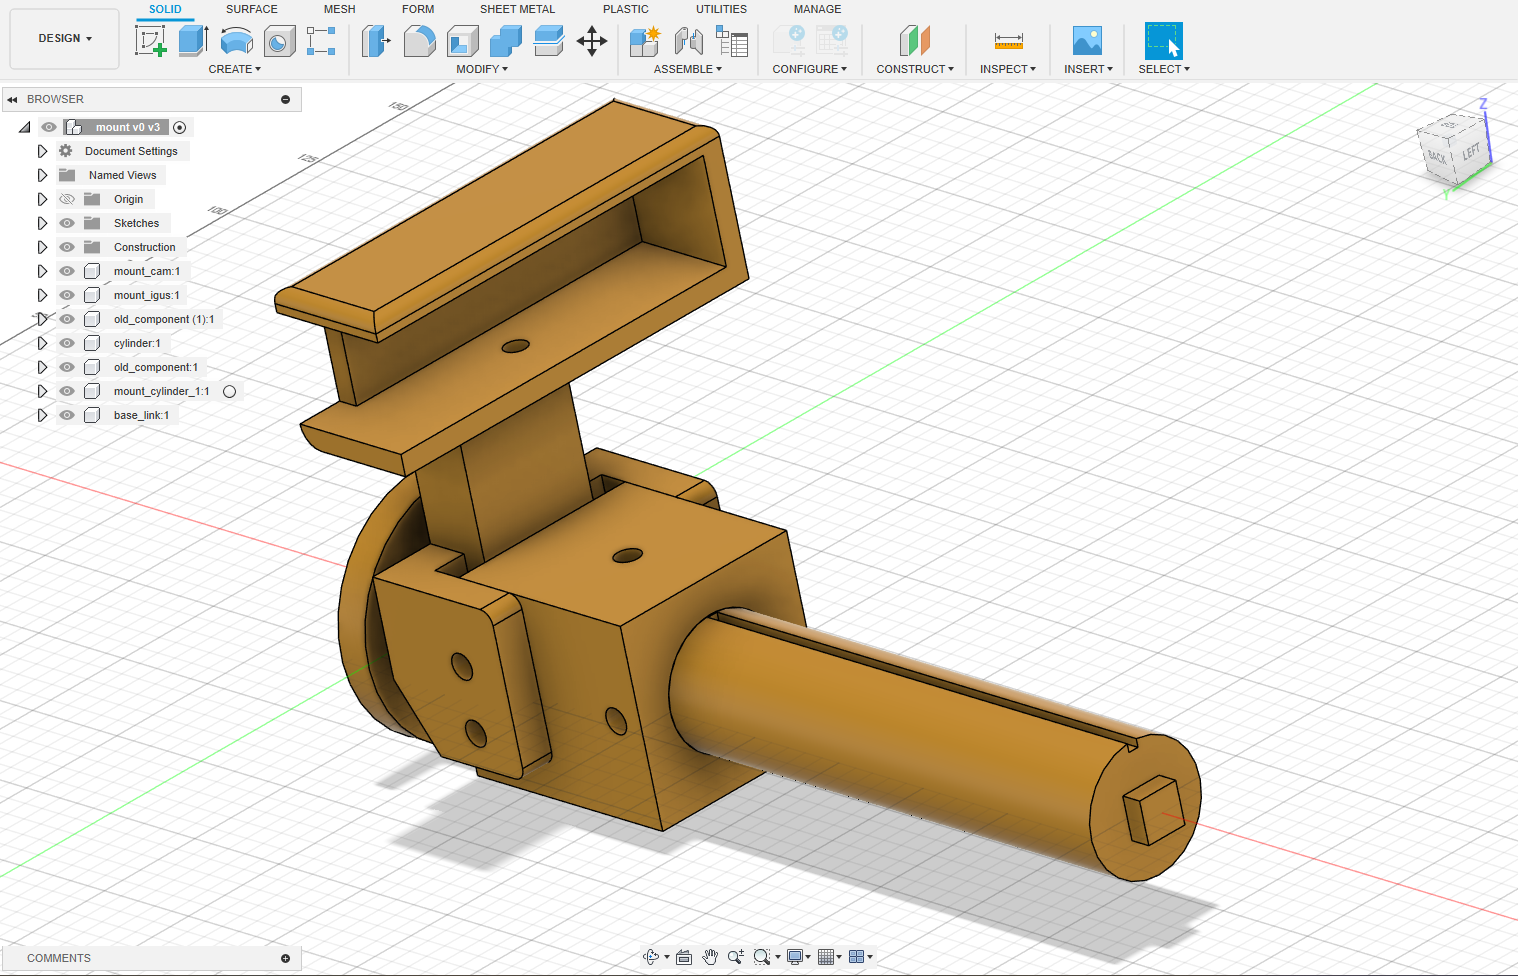
\includegraphics[width=0.45\textwidth]{c3_23.png}
    \caption{MountV1 with cylinder presser}
    \label{fig:mountv1}
\end{figure}

\begin{figure}[H]
    \centering
    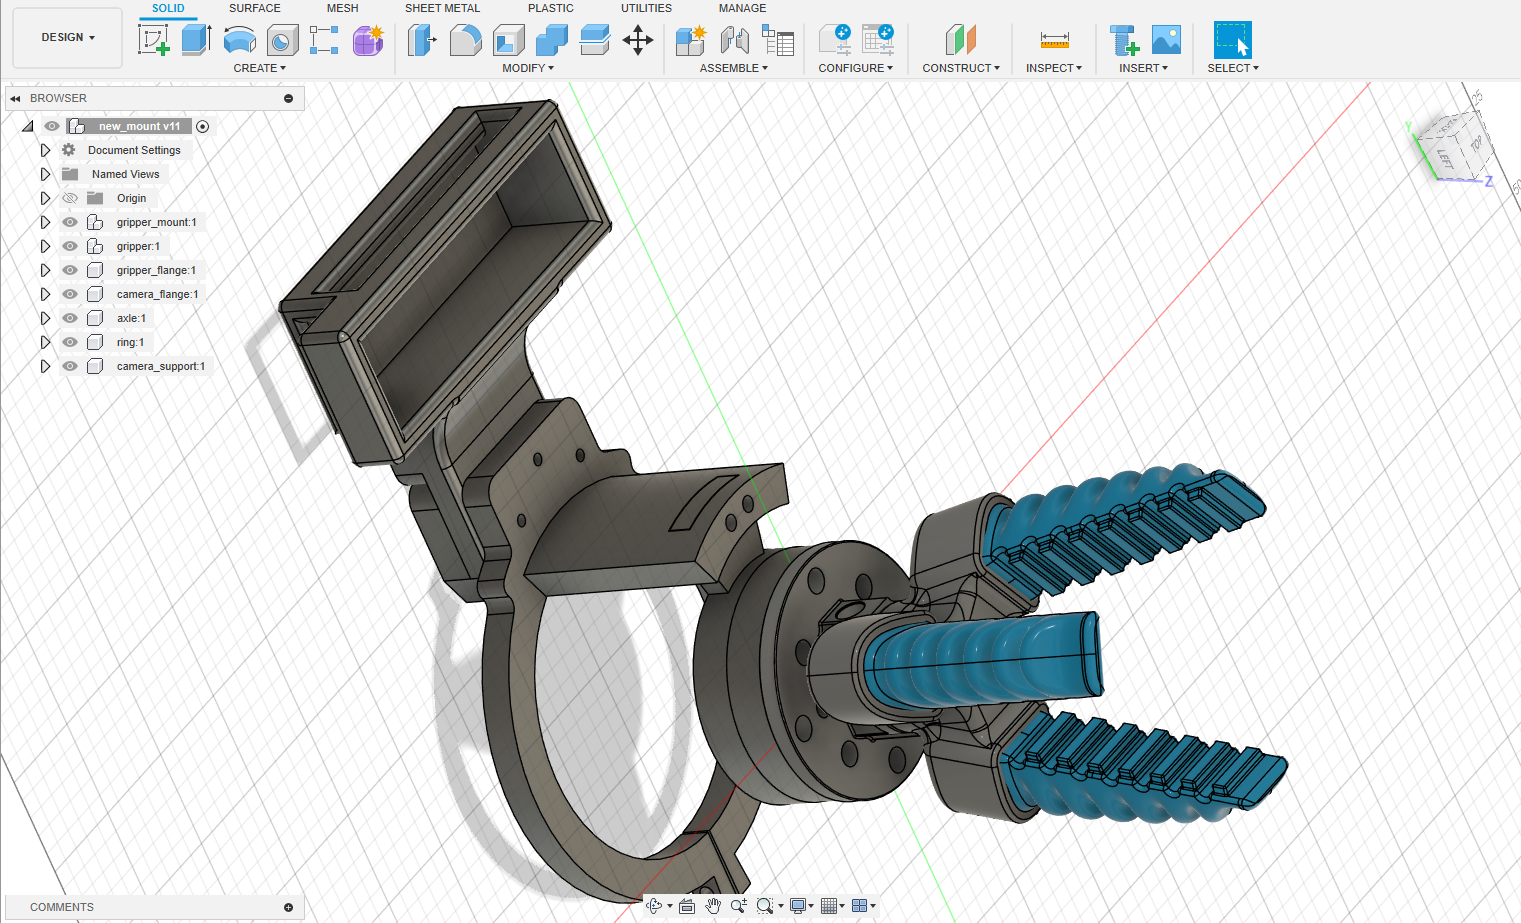
\includegraphics[width=0.45\textwidth]{c3_24.png}
    \caption{Mountv2 with soft gripper}
    \label{fig:mountv2}
\end{figure}

Power management involves DC/DC converters to power the onboard computer and sensors from the mobile robot's 
internal battery. External lead batteries power the robotic arm and pneumatic pump, with Molex connectors enabling
easy switching between battery packs and the external power supply.

The ReBeL cobot presented challenges due to its low-cost design. The motor encoders lacked accuracy and repeatability,
and the plastic gears exhibited backlash and deformation under load. These issues were addressed with artificial 
error compensation and careful calibration procedures.
Additionally, the Intel RealSense camera required calibration using the manufacturer's software to ensure accurate
depth estimation and object localization.

Overall, this mobile manipulation platform represents a functional and adaptable solution for various applications 
in industrial and agricultural settings. The integration of diverse hardware and software components, combined with
rigorous testing, demonstrates the system's potential for real-world automation tasks.
Figure \ref{fig:setup} shows a picture of the complete setup of the mobile manipulation robot.

\begin{figure}[H]
    \centering
    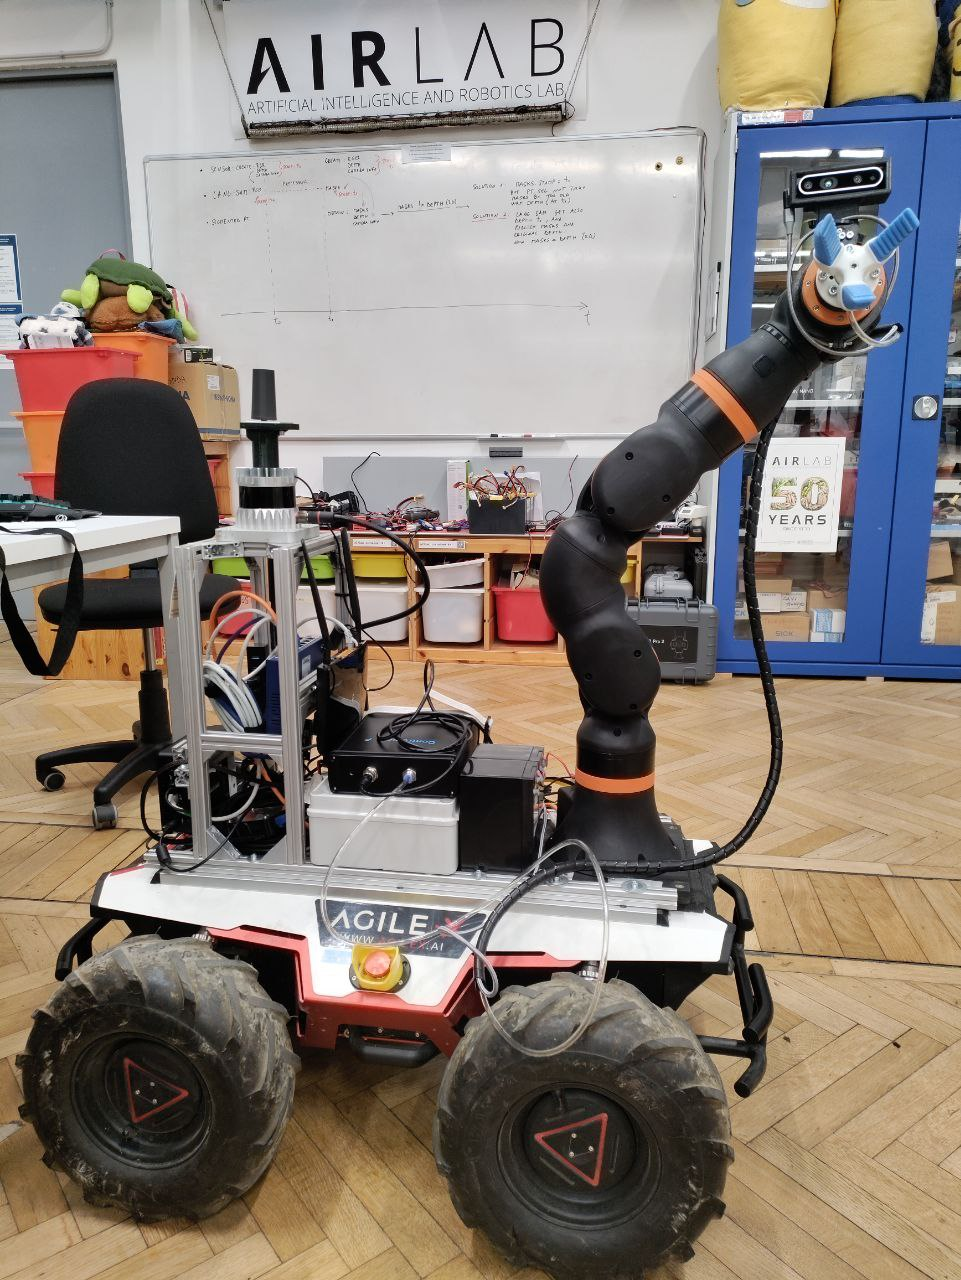
\includegraphics[width=0.45\textwidth]{c3_28.jpg}
    \caption{Mobile Manipulator Robot Setup}
    \label{fig:setup}
\end{figure}

\section{Software Architecture and Control}

The system leverages the Robot Operating System 2 (ROS2) as the middleware, providing a flexible framework for
integrating diverse software components and enabling communication between nodes.

A key aspect of the software development was creating a ROS2 control interface for the Igus Rebel arm, enabling 
high-level control and monitoring through the Ethernet interface. This interface interacts with the Joint Trajectory 
Controller, which receives motion plans from MoveIt2 and translates them into joint positions or velocities for 
the arm's motors. The implementation relies on the ROS2-Control framework and a custom hardware interface designed
for the Igus Rebel arm.

MoveIt2, a powerful motion planning framework, plays a central role in planning and executing arm trajectories. 
Its modular architecture, consisting of components like the Planning Scene, Planning Pipeline libraries, and 
Kinematics Solver, facilitates seamless integration with ROS2. A custom ROS2 library simplifies the use of 
MoveIt2 for the Igus Rebel arm, offering high-level functions for planning and executing various types of motion.

The RViz2 visualization tool allows for real-time visualization of the robot's motion in both simulated and real 
environments. It aids in debugging and validating the functionality of the software components, including the 
kinematic model, planning scene, and motion plans, as shown in Figure \ref{fig:moveit2}.

To address the challenges of collision avoidance in dynamic environments, the Octomap library is integrated with
MoveIt2. Octomap generates 3D occupancy maps of the surroundings, enabling the robot to avoid obstacles. 
However, due to the ongoing development of the Octomap library for ROS2, limitations such as slow updates and 
false positives in collision checking were encountered.

\begin{figure}[H]
    \centering
    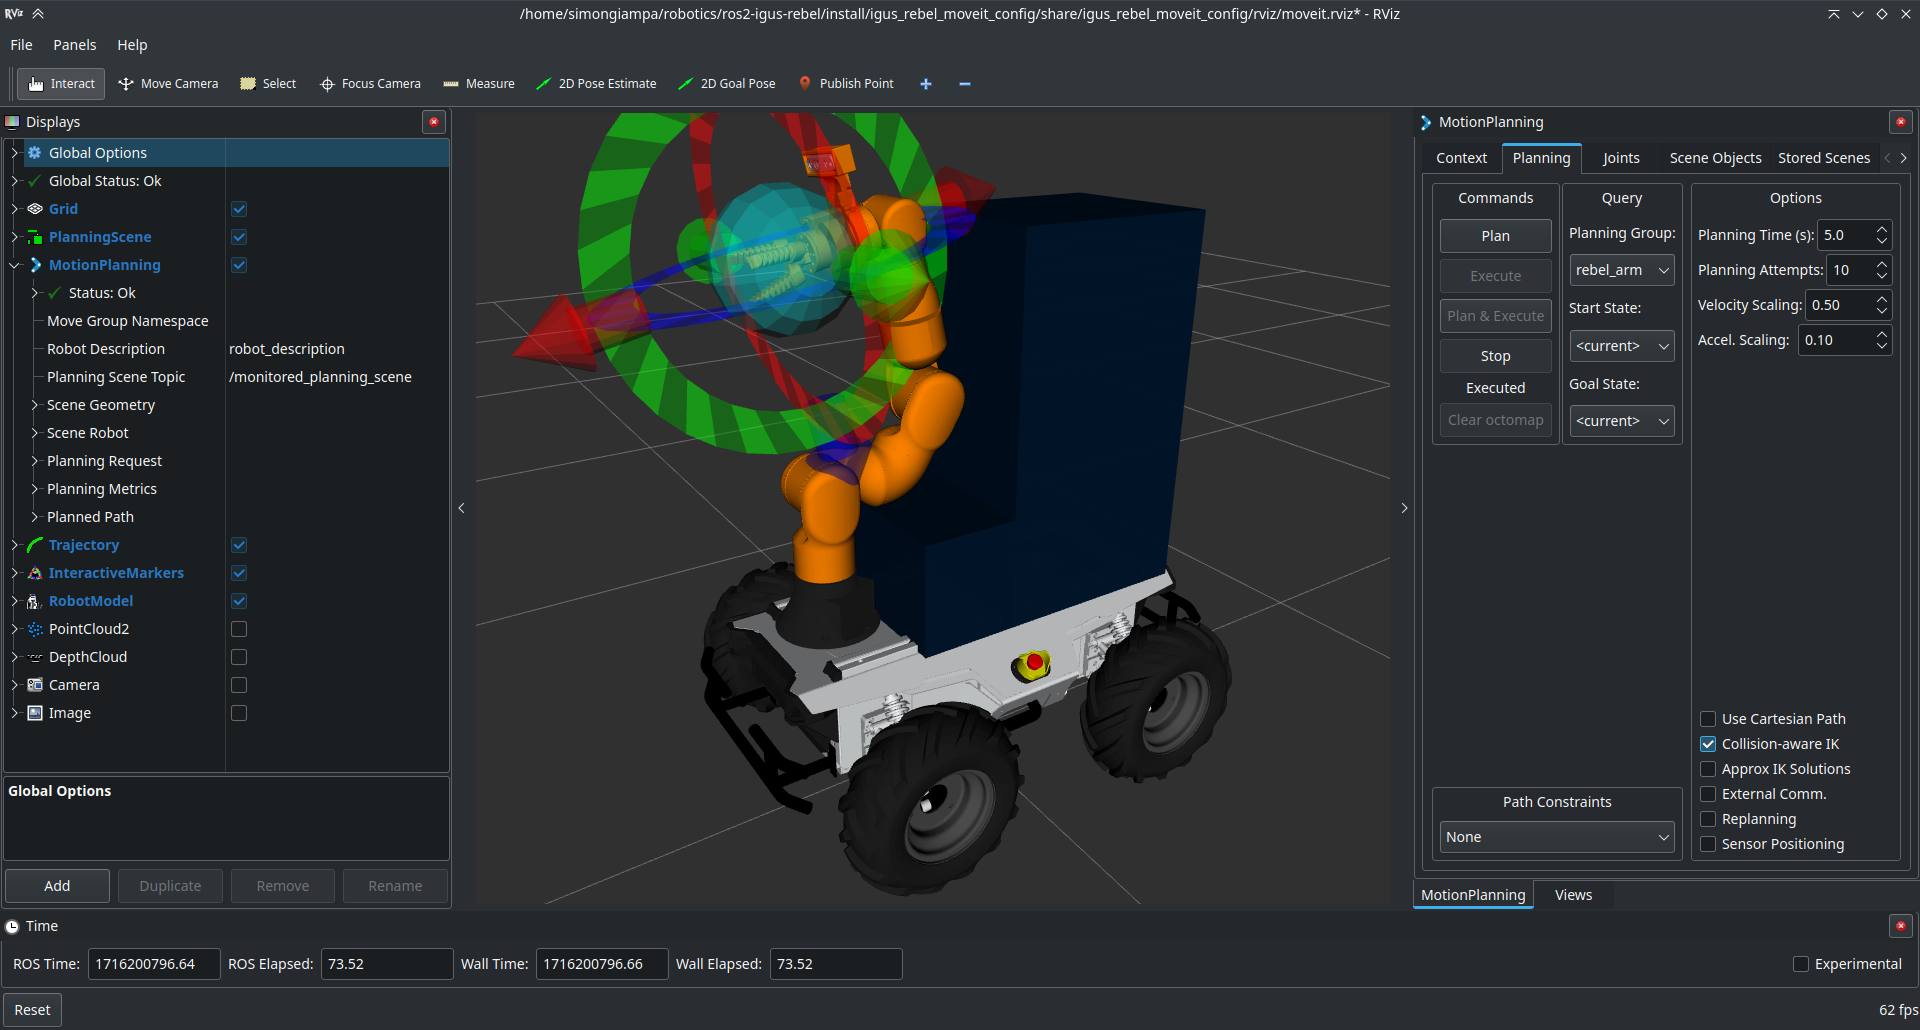
\includegraphics[width=0.45\textwidth]{c4_11.png}
    \caption{RViz2 visualization of MoveIt2 planning scene}
    \label{fig:moveit2}
\end{figure}

Actuation of the soft gripper is achieved through a ROS2-control interface that communicates with an Arduino UNO
microcontroller. This microcontroller controls the pneumatic pump responsible for opening and closing the gripper's fingers.
Serial communication over the UART protocol facilitates this control, allowing for precise actuation of the soft
gripper during manipulation tasks.

The Ignition Gazebo simulation environment serves as a crucial tool for testing and refining the robot's navigation
and manipulation capabilities. A realistic warehouse environment with various obstacles was created to validate 
the performance of the Nav2 navigation framework and associated algorithms in a safe and controlled setting,
as shown in Figure \ref{fig:ignition}.

\begin{figure}[H]
    \centering
    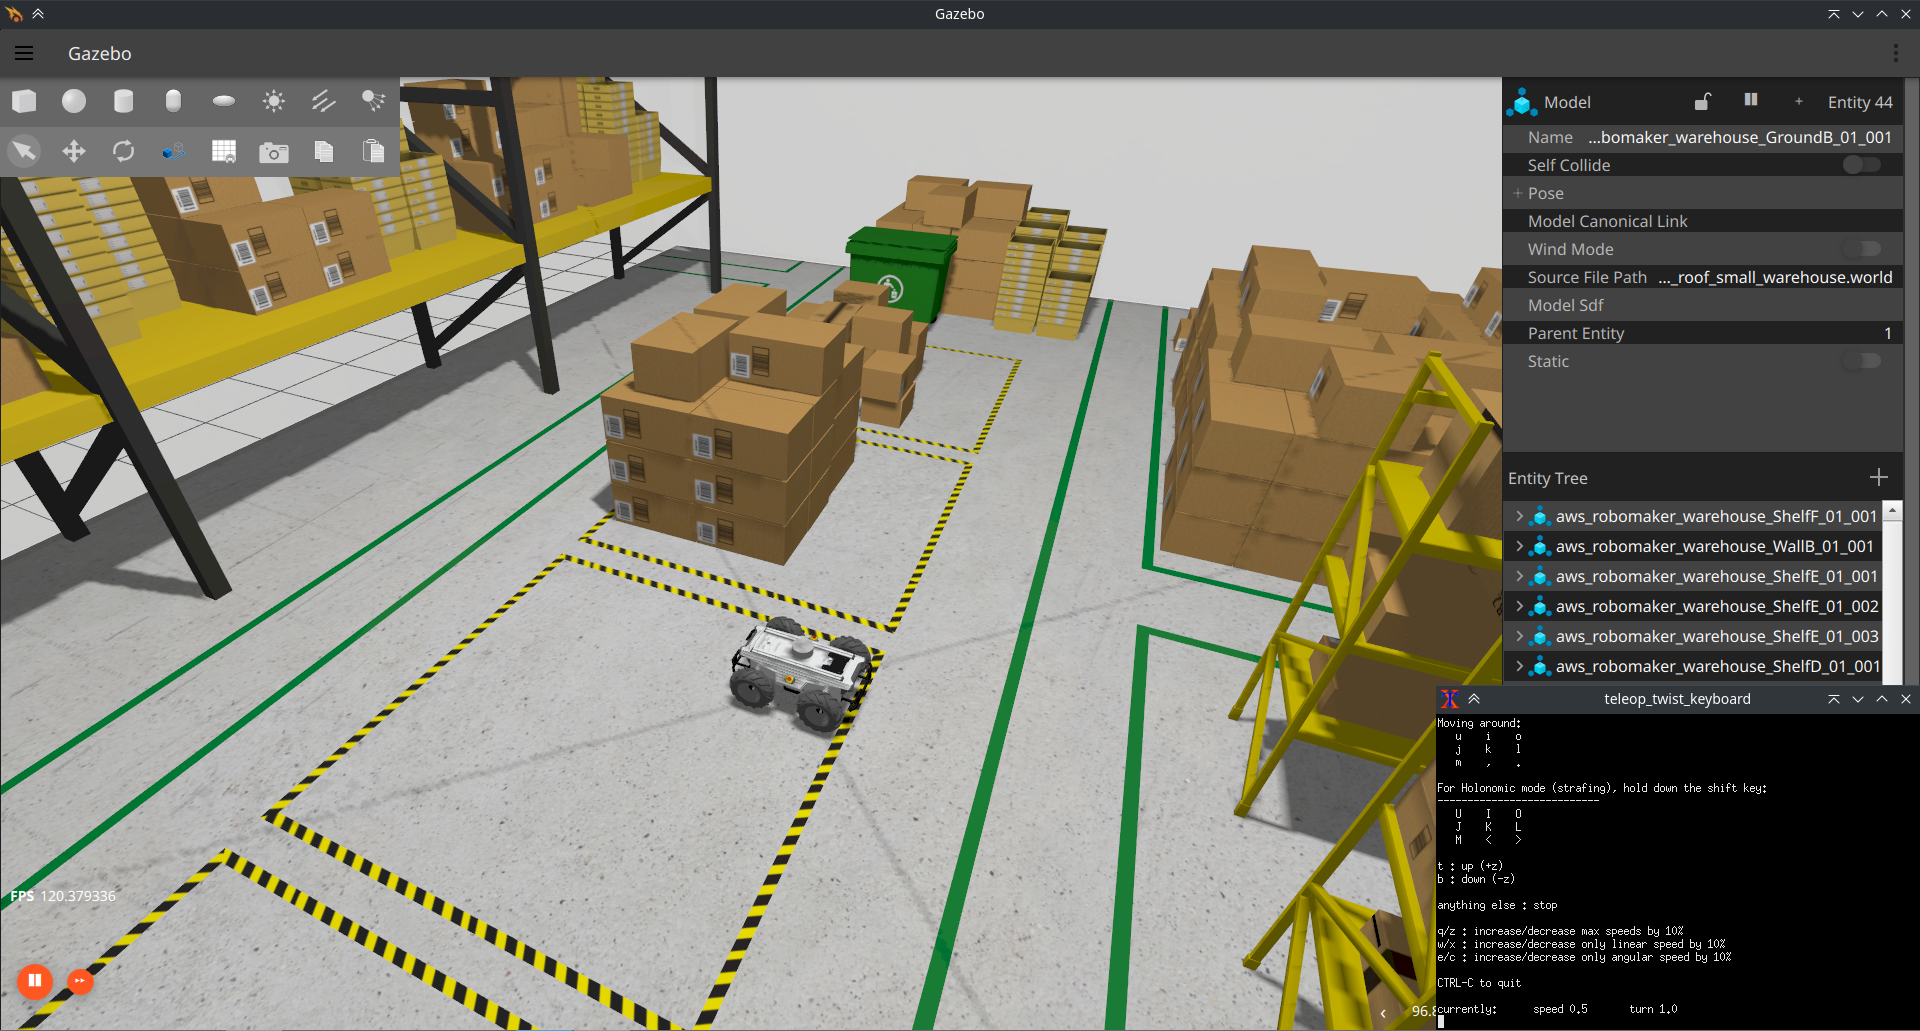
\includegraphics[width=0.45\textwidth]{c4_12.png}
    \caption{Ignition Gazebo Simulation Environment for the mobile robot base}
    \label{fig:ignition}
\end{figure}

Nav2, a comprehensive software framework for autonomous navigation, is utilized for planning and executing the mobile
robot's trajectories. Its modular architecture accommodates various plugins, including costmap layers, localizers,
planners, and recovery behaviors. SLAM Toolbox is employed for mapping and localization, while the Hybrid A* 
global planner and MPPI local planner ensure efficient and collision-free navigation.

Parameter tuning in Nav2 was a significant undertaking, requiring extensive testing in both simulated and real 
environments to achieve optimal performance. Adjustments were made to localization algorithms, global and local
planners, recovery behaviors, and costmap configurations to ensure safe and reliable navigation in diverse 
scenarios.

A notable challenge encountered during testing was the low and unreliable frequency of the LiDAR sensor. 
This issue, stemming from a combination of network congestion and the default DDS middleware configuration, 
was resolved by reconfiguring the middleware to prioritize local communication and adopting the Cyclone DDS 
implementation. This optimization significantly improved data transmission and overall system stability.

A parking algorithm was designed to enable the mobile robot to autonomously position itself optimally
for manipulation tasks. The algorithm considers the target location, costmap, and robot footprint to generate 
candidate poses and select the most suitable one based on a ranking function. Despite its effectiveness in most 
cases, the algorithm's limitations, primarily related to the robot arm's workspace approximation, highlight
potential areas for future refinement.

ArUco markers are utilized for precise object localization and pose estimation. 
Detection involves identifying the marker's corners and ID using the OpenCV ArUco library, while pose estimation
utilizes these corners, marker size, and camera intrinsic parameters to determine the marker's position and
orientation relative to the camera.

To overcome challenges in estimating the orientation of small ArUco markers, a multi-ArUco plane estimation 
algorithm was developed. This algorithm assumes the coplanarity of multiple markers and utilizes RANSAC, 
least squares estimation, PCA, and SVD to determine the plane's orientation, thus refining the individual 
marker poses.

The YOLOv8 object detection model, a state-of-the-art real-time algorithm, was employed for detecting colored
balls and apples in the environment, as demonstrated in Figure \ref{fig:yolov8}.
Trained on a custom dataset with augmented images, YOLOv8 achieved 
satisfactory performance in terms of mean Average Precision (mAP) and Intersection over Union (IoU).
Challenges with high false positive rates were addressed by adjusting the confidence threshold.

\begin{figure}[H]
    \centering
    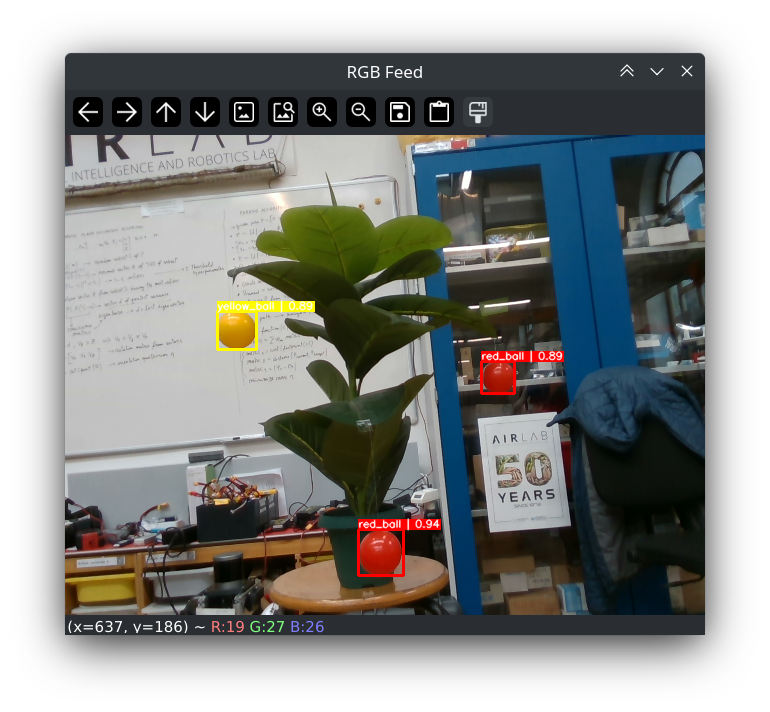
\includegraphics[width=0.45\textwidth]{c4_16.png}
    \caption{YOLOv8 Inference in action}
    \label{fig:yolov8}
\end{figure}

The object's pose estimation process combines object detection with depth perception from the RealSense camera.
A segmented point cloud is created by filtering the depth map based on the detected object's bounding box and color mask.
The object's center is estimated by fitting a sphere to the segmented point cloud using RANSAC and MLESAC algorithms,
enabling the calculation of an optimal grasping pose for the robotic arm.

Two algorithms, sphere barycenter estimation and grasp pose estimation, facilitate the manipulation of objects. The former estimates the object's center from the segmented point cloud, assuming a spherical shape, 
while the latter generates candidate grasping poses and selects the most suitable one based on inverse kinematics 
feasibility and a heuristic ranking. This approach is simplified due to the compliance of the soft gripper fingers, 
allowing for some error in pose estimation.

Collision avoidance is achieved using the Octomap library, which generates 3D occupancy maps based on sensor data. 
However, the current ROS2 implementation of Octomap has limitations in updating and maintaining accurate 
representations of dynamic environments, leading to potential false positives in collision detection.

To control the soft gripper, a ROS2-control interface communicates with an Arduino UNO microcontroller, 
which in turn controls the pneumatic pump responsible for actuating the gripper's fingers. 
This serial communication setup ensures precise control over the grasping action.

The experimental setups involved both simulated and real-world scenarios. A simulated warehouse environment
in Ignition Gazebo was used to test and validate the navigation and obstacle avoidance algorithms. 
Additionally, artificial plants with colored balls and apples served as realistic environments for testing
the object picking capabilities of the mobile manipulator.

The ROS2 Actions client-server architecture provides a modular and scalable framework for implementing high-level tasks.
It enables efficient communication and coordination between different software components, 
ensuring robust and reliable execution of complex behaviors like autonomous navigation, object detection, grasping,
and manipulation.

The integration of ROS2, MoveIt2, Nav2, and other components 
has resulted in a capable and adaptable system ready for deployment in real-world scenarios. Future work could focus
on improving the integration of Octomap with MoveIt2, refining the grasping algorithms for the soft gripper, 
and exploring more advanced perception techniques to enhance the robot's capabilities further.

\section{Experimental Setups and Demonstrations}

Experimental setups and demonstrations were designed to showcase the capabilities of the 
mobile manipulation robot in industrial and agricultural scenarios. Three distinct demonstrations were conducted:
the ArUco Follower, the Button Presser, and the Object Picking demos.

The ArUco Follower demo served as a preliminary test for the robotic arm's autonomous control software. 
Utilizing the MoveIt2 motion planning framework and ArUco marker detection and pose estimation algorithms, 
the robot arm successfully tracked and followed a moving ArUco marker with its end effector. However, 
attempts to integrate the MoveIt2 Servo node for real-time control proved challenging due to stability issues
and the need for precise PID tuning.

The Button Presser demo highlighted the robot's potential in industrial settings by demonstrating its ability 
to autonomously press buttons on a custom-designed control panel. Two iterations of the end-effector mount were employed,
with MountV2 incorporating a vacuum suction cap to enhance button-pressing reliability. The demo involved a 
sequence of steps, including navigating to the control panel, detecting ArUco markers with the 
multi-ArUco plane estimation algorithm to locate the buttons, 
and executing planned trajectories to press them in a predefined order. Figure \ref{fig:buttonpresser} shows the robot
while interacting with the control panel.

\begin{figure}[H]
    \centering
    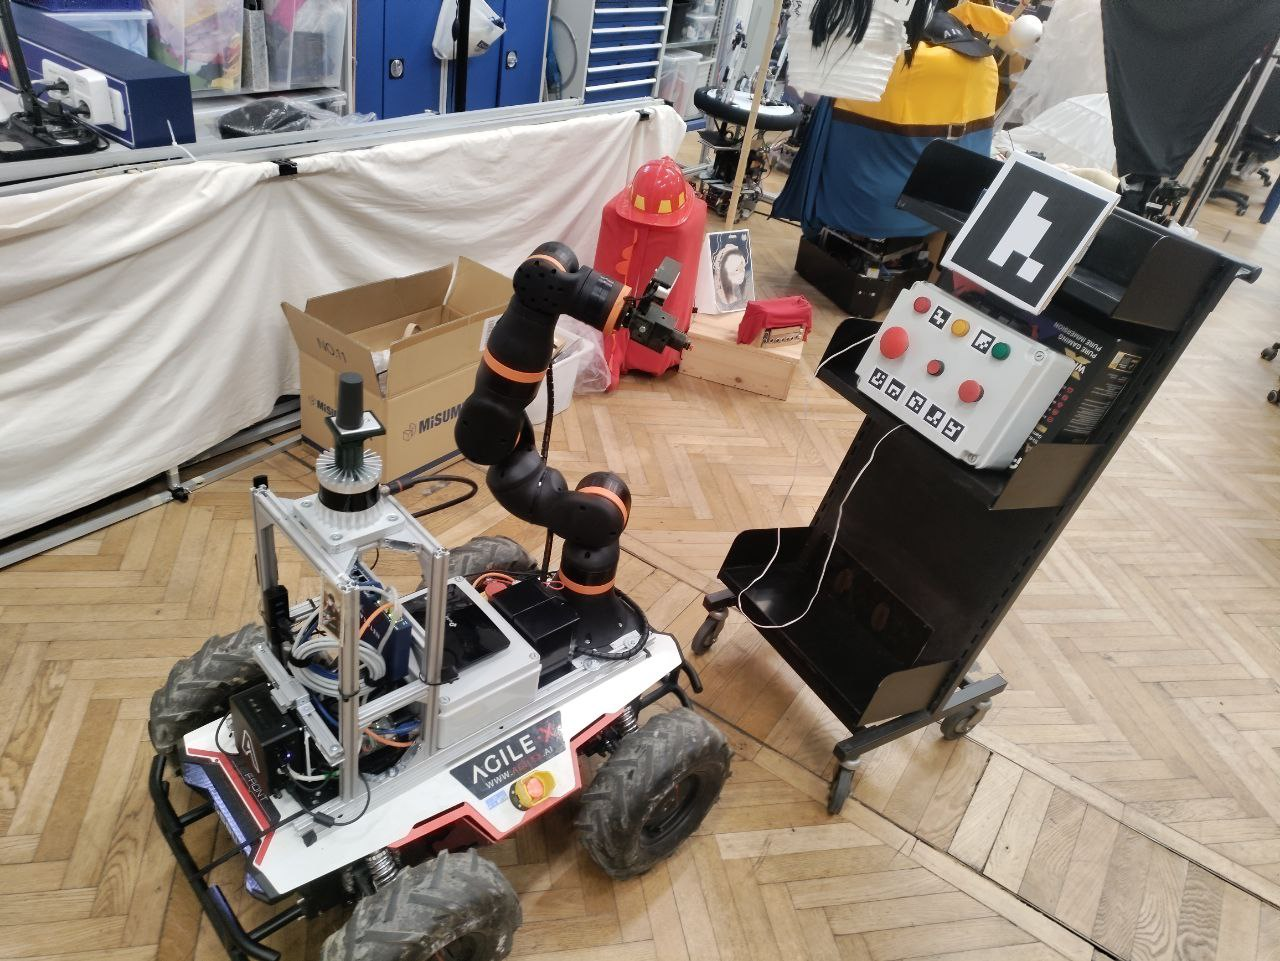
\includegraphics[width=0.45\textwidth]{c5_10.jpg}
    \caption{Mobile Button Presser Demo}
    \label{fig:buttonpresser}
\end{figure}

The Object Picking demo showcased the robot's adaptability in agricultural scenarios, specifically focusing 
on picking colored balls and apples from artificial plants. The demo utilized the YOLOv8 object detection model,
trained on a custom dataset, to identify and locate objects.
Two versions of the Object Picking demo were implemented. In the first version, the robot picked objects and 
placed them in a basket mounted on the mobile base. The second version involved navigating to a separate dropping 
location, requiring the robot to utilize its navigation and obstacle avoidance capabilities. Both versions 
successfully demonstrated the robot's ability to autonomously pick and place objects in a simulated agricultural 
environment. Figure \ref{fig:demo2_1} shows the robot picking apples from an artificial plant, 
while Figure \ref{fig:demo2_2} depicts the robot dropping a picked apple in the designated location.

\begin{figure}[H]
    \centering
    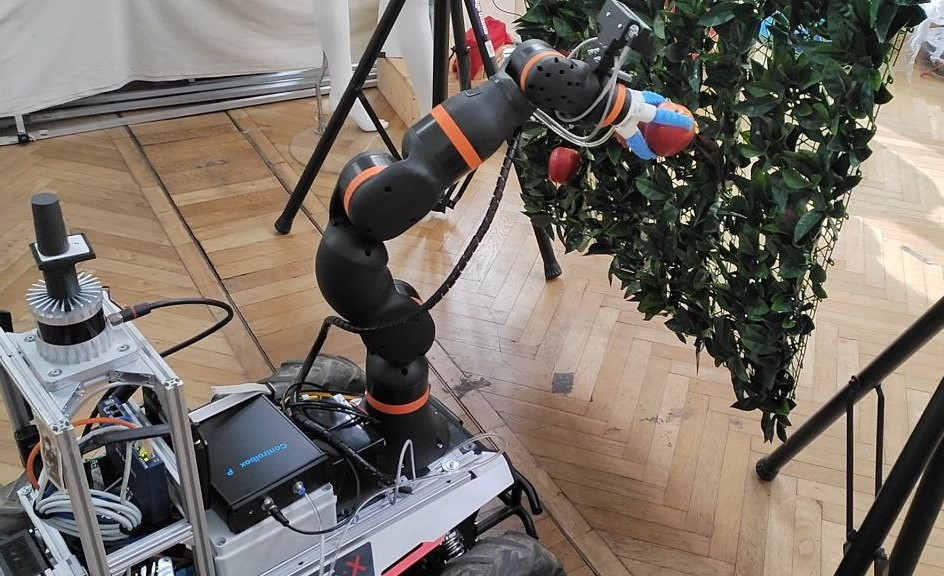
\includegraphics[width=0.45\textwidth]{c5_17.jpg}
    \caption{Mobile Fruit Picking Demo: Object Picking Version 2 while picking apples from an artificial plant}
    \label{fig:demo2_1}
\end{figure}

\begin{figure}[H]
    \centering
    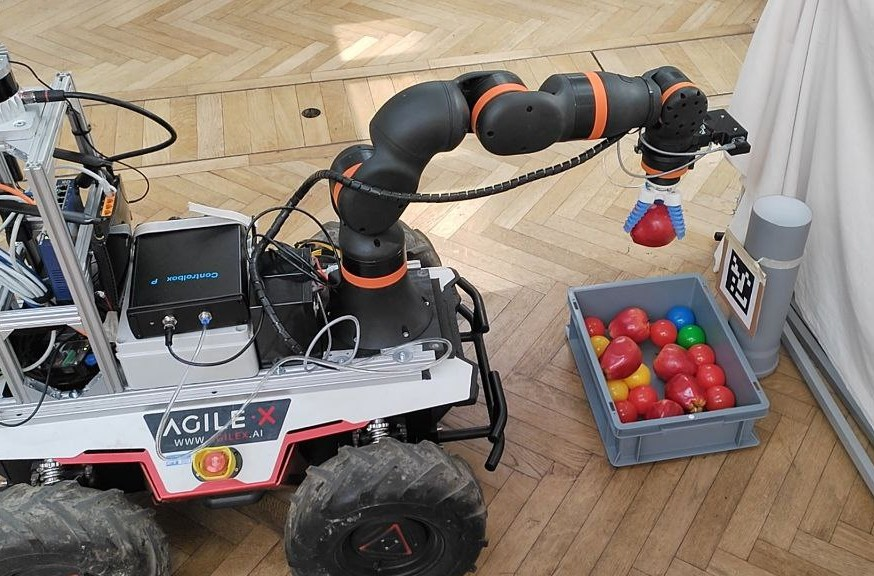
\includegraphics[width=0.45\textwidth]{c5_18.jpg}
    \caption{Mobile Fruit Picking Demo: Object Picking Version 2 while dropping a picked apple}
    \label{fig:demo2_2}
\end{figure}

The object picking routine, common to both versions, involved generating a list of waypoints for the robot to follow,
detecting objects at each waypoint, computing priority scores for detected objects based on distance and confidence, 
estimating object centers using a RANSAC sphere fitting algorithm, and calculating grasping poses. The robot then 
executed trajectories to approach, grasp, and transport the object to the designated dropping location.

The implementation of these demos relied heavily on the ROS2 framework, leveraging its action client-server 
architecture for high-level task coordination. The system architecture encompassed various components, including 
MoveIt2 servers for planning and execution, Nav2 servers for navigation, a client 
node for orchestration, a neural network node for object detection, and an ArUco pose estimation node.

Throughout the development and testing of these demos, several challenges were encountered. These included 
dealing with the infrared reflectivity of objects, the slow inference speed of the object detection network, 
and the limitations of the Octomap library for collision avoidance. Workarounds and optimizations were 
implemented to mitigate these issues, demonstrating the resilience and adaptability of the robotic system.

Overall, these experimental setups and demonstrations showcase the potential of the mobile manipulation robot
for autonomous operation in both industrial and agricultural settings. They highlight the successful integration 
of diverse software components, including perception, motion planning, grasping, and navigation, into a 
unified system capable of performing complex tasks.  The results of these experiments provide valuable insights
for future research and development in mobile manipulation robotics, paving the way for more sophisticated 
and versatile autonomous systems.

%-----------------------------------------------------------------------------
% CONCLUSION
%-----------------------------------------------------------------------------
\section{Conclusions}

This thesis has successfully demonstrated the feasibility of developing a cost-effective, autonomous mobile 
manipulation robot for industrial and agricultural applications. By integrating a mobile platform with a robotic
arm and utilizing ROS2, Nav2, and MoveIt2 frameworks, the system achieved autonomous navigation, object manipulation, 
and task execution in dynamic environments. A key contribution was the design and implementation of a pneumatic 
soft gripper, showcasing its potential for delicate object handling.

Through rigorous testing in simulated and real-world scenarios, the project highlighted the importance of robust 
perception, localization, and sensor fusion in achieving reliable performance. The modular software architecture 
and comprehensive documentation facilitate future research and development, enabling further refinement and 
extension of the system's capabilities.

This research lays the groundwork for advancing mobile manipulation robotics. Future endeavors could focus on 
enhancing perception algorithms, exploring deep learning techniques for object recognition and grasping, and 
integrating ROS2 behavior trees for more complex task planning. Ultimately, this project contributes to the 
vision of creating adaptable and intelligent robotic systems that can revolutionize industries by automating 
complex tasks and improving efficiency and safety.

%-----------------------------------------------------------------------------
% IMAGES names to place

% c3_23 mountv1
% c3_24 mountv2
% c3_28 complete robot setup
% c4_11 moveit2 RViz2
% c4_12 gazebo 
% c4_16 yolov8
% c5_10 button presser demo
% c5_17, c5_18 mobile fruit picking demo

%---------------------------------------------------------------------------
%  BIBLIOGRAPHY
%---------------------------------------------------------------------------
% Remember to insert here only the essential bibliography of your work
\bibliography{chapters/biblio.bib} % automatically inserted and ordered with this command 


\end{document}